\documentclass[ignorenonframetext,]{beamer}
\setbeamertemplate{caption}[numbered]
\setbeamertemplate{caption label separator}{: }
\setbeamercolor{caption name}{fg=normal text.fg}
\beamertemplatenavigationsymbolsempty
\usepackage{lmodern}
\usepackage{amssymb,amsmath}
\usepackage{ifxetex,ifluatex}
\usepackage{fixltx2e} % provides \textsubscript
\ifnum 0\ifxetex 1\fi\ifluatex 1\fi=0 % if pdftex
  \usepackage[T1]{fontenc}
  \usepackage[utf8]{inputenc}
\else % if luatex or xelatex
  \ifxetex
    \usepackage{mathspec}
  \else
    \usepackage{fontspec}
  \fi
  \defaultfontfeatures{Ligatures=TeX,Scale=MatchLowercase}
\fi
% use upquote if available, for straight quotes in verbatim environments
\IfFileExists{upquote.sty}{\usepackage{upquote}}{}
% use microtype if available
\IfFileExists{microtype.sty}{%
\usepackage{microtype}
\UseMicrotypeSet[protrusion]{basicmath} % disable protrusion for tt fonts
}{}
\newif\ifbibliography
\hypersetup{
            pdftitle={Models and Markets},
            pdfauthor={Kiernan Nicholls},
            pdfborder={0 0 0},
            breaklinks=true}
\urlstyle{same}  % don't use monospace font for urls
\usepackage{color}
\usepackage{fancyvrb}
\newcommand{\VerbBar}{|}
\newcommand{\VERB}{\Verb[commandchars=\\\{\}]}
\DefineVerbatimEnvironment{Highlighting}{Verbatim}{commandchars=\\\{\}}
% Add ',fontsize=\small' for more characters per line
\usepackage{framed}
\definecolor{shadecolor}{RGB}{248,248,248}
\newenvironment{Shaded}{\begin{snugshade}}{\end{snugshade}}
\newcommand{\KeywordTok}[1]{\textcolor[rgb]{0.13,0.29,0.53}{\textbf{#1}}}
\newcommand{\DataTypeTok}[1]{\textcolor[rgb]{0.13,0.29,0.53}{#1}}
\newcommand{\DecValTok}[1]{\textcolor[rgb]{0.00,0.00,0.81}{#1}}
\newcommand{\BaseNTok}[1]{\textcolor[rgb]{0.00,0.00,0.81}{#1}}
\newcommand{\FloatTok}[1]{\textcolor[rgb]{0.00,0.00,0.81}{#1}}
\newcommand{\ConstantTok}[1]{\textcolor[rgb]{0.00,0.00,0.00}{#1}}
\newcommand{\CharTok}[1]{\textcolor[rgb]{0.31,0.60,0.02}{#1}}
\newcommand{\SpecialCharTok}[1]{\textcolor[rgb]{0.00,0.00,0.00}{#1}}
\newcommand{\StringTok}[1]{\textcolor[rgb]{0.31,0.60,0.02}{#1}}
\newcommand{\VerbatimStringTok}[1]{\textcolor[rgb]{0.31,0.60,0.02}{#1}}
\newcommand{\SpecialStringTok}[1]{\textcolor[rgb]{0.31,0.60,0.02}{#1}}
\newcommand{\ImportTok}[1]{#1}
\newcommand{\CommentTok}[1]{\textcolor[rgb]{0.56,0.35,0.01}{\textit{#1}}}
\newcommand{\DocumentationTok}[1]{\textcolor[rgb]{0.56,0.35,0.01}{\textbf{\textit{#1}}}}
\newcommand{\AnnotationTok}[1]{\textcolor[rgb]{0.56,0.35,0.01}{\textbf{\textit{#1}}}}
\newcommand{\CommentVarTok}[1]{\textcolor[rgb]{0.56,0.35,0.01}{\textbf{\textit{#1}}}}
\newcommand{\OtherTok}[1]{\textcolor[rgb]{0.56,0.35,0.01}{#1}}
\newcommand{\FunctionTok}[1]{\textcolor[rgb]{0.00,0.00,0.00}{#1}}
\newcommand{\VariableTok}[1]{\textcolor[rgb]{0.00,0.00,0.00}{#1}}
\newcommand{\ControlFlowTok}[1]{\textcolor[rgb]{0.13,0.29,0.53}{\textbf{#1}}}
\newcommand{\OperatorTok}[1]{\textcolor[rgb]{0.81,0.36,0.00}{\textbf{#1}}}
\newcommand{\BuiltInTok}[1]{#1}
\newcommand{\ExtensionTok}[1]{#1}
\newcommand{\PreprocessorTok}[1]{\textcolor[rgb]{0.56,0.35,0.01}{\textit{#1}}}
\newcommand{\AttributeTok}[1]{\textcolor[rgb]{0.77,0.63,0.00}{#1}}
\newcommand{\RegionMarkerTok}[1]{#1}
\newcommand{\InformationTok}[1]{\textcolor[rgb]{0.56,0.35,0.01}{\textbf{\textit{#1}}}}
\newcommand{\WarningTok}[1]{\textcolor[rgb]{0.56,0.35,0.01}{\textbf{\textit{#1}}}}
\newcommand{\AlertTok}[1]{\textcolor[rgb]{0.94,0.16,0.16}{#1}}
\newcommand{\ErrorTok}[1]{\textcolor[rgb]{0.64,0.00,0.00}{\textbf{#1}}}
\newcommand{\NormalTok}[1]{#1}
\usepackage{graphicx,grffile}
\makeatletter
\def\maxwidth{\ifdim\Gin@nat@width>\linewidth\linewidth\else\Gin@nat@width\fi}
\def\maxheight{\ifdim\Gin@nat@height>\textheight0.8\textheight\else\Gin@nat@height\fi}
\makeatother
% Scale images if necessary, so that they will not overflow the page
% margins by default, and it is still possible to overwrite the defaults
% using explicit options in \includegraphics[width, height, ...]{}
\setkeys{Gin}{width=\maxwidth,height=\maxheight,keepaspectratio}

% Prevent slide breaks in the middle of a paragraph:
\widowpenalties 1 10000
\raggedbottom

\AtBeginPart{
  \let\insertpartnumber\relax
  \let\partname\relax
  \frame{\partpage}
}
\AtBeginSection{
  \ifbibliography
  \else
    \let\insertsectionnumber\relax
    \let\sectionname\relax
    \frame{\sectionpage}
  \fi
}
\AtBeginSubsection{
  \let\insertsubsectionnumber\relax
  \let\subsectionname\relax
  \frame{\subsectionpage}
}

\setlength{\parindent}{0pt}
\setlength{\parskip}{6pt plus 2pt minus 1pt}
\setlength{\emergencystretch}{3em}  % prevent overfull lines
\providecommand{\tightlist}{%
  \setlength{\itemsep}{0pt}\setlength{\parskip}{0pt}}
\setcounter{secnumdepth}{0}

\title{Models and Markets}
\subtitle{Comparing Predictive Capabilities}
\author{Kiernan Nicholls}
\date{December 4, 2018}

\begin{document}
\frame{\titlepage}

\begin{frame}{Why predict elections?}

\begin{itemize}
\tightlist
\item
  Resource allocation
\item
  Strategy adjustment
\item
  Quantitative journalism
\item
  Uncertainty is scary
\end{itemize}

\end{frame}

\begin{frame}{How to Predict Elections}

\begin{enumerate}
\def\labelenumi{\arabic{enumi}.}
\tightlist
\item
  Opinion polling
\item
  Polling aggregation
\item
  Forecast modeling
\item
  Prediction markets
\end{enumerate}

\end{frame}

\begin{frame}{Opion Polling}

\emph{e.g., Washington Post/ABC}

In 1824 \emph{The Harrisburg Pennsylvanian} had Jackson over Adams, 335
to 169.

\begin{itemize}
\tightlist
\item
  Sample Size
\item
  Methodology
\item
  Partisanship
\end{itemize}

\end{frame}

\begin{frame}{Polling Aggrigation}

\emph{e.g., RealClearPolitics}

\begin{itemize}
\tightlist
\item
  21st century invention
\item
  Average out all polls
\item
  Minimize errors and reduce bias
\item
  Possibly weighted
\end{itemize}

\end{frame}

\begin{frame}{Forecasting Models}

Montel carlo simulations = probability distribution

\begin{enumerate}
\def\labelenumi{\arabic{enumi}.}
\tightlist
\item
  Define a domain of possible inputs
\item
  Generate inputs randomly from a probability distribution over the
  domain
\item
  Perform a deterministic computation on the inputs
\item
  Aggregate the results
\end{enumerate}

\begin{itemize}
\tightlist
\item
  Poll, average, deviation
\item
  20,000 interations
\item
  Law of large numbers
\end{itemize}

\end{frame}

\begin{frame}{About FiveThirtyEight}

\begin{itemize}
\tightlist
\item
  Founded in 2008, sold to NYT then ABC
\item
  Least inaccurate in 2016 (Clinton @ 71\%)
\end{itemize}

\begin{quote}
Someone could look like a genius simply by doing some fairly basic
research into what really has predictive power in a political campaign
\end{quote}

\begin{quote}
--- Nate Silver
\end{quote}

\end{frame}

\begin{frame}{FiveThirtyEight Forecast}

\begin{quote}
It takes lots of polls, performs various types of adjustments to them,
and then blends them with other kinds of empirically useful
indicators\ldots{} Then it accounts for the uncertainty in the forecast
and simulates the election thousands of times.
\end{quote}

\begin{enumerate}
\def\labelenumi{\arabic{enumi}.}
\tightlist
\item
  \textbf{Polling}: District-by-district polling, adjusted for house
  effects and other factors.
\item
  \textbf{CANTOR}: Infers results for districts with little or no
  polling from comparable districts with polling.
\item
  \textbf{Fundamentals}: District partisanship, past performance,
  generic ballot, fundraising, experience, scandals
\end{enumerate}

\end{frame}

\begin{frame}[fragile]{Model Data}

\begin{verbatim}
## # A tibble: 89,918 x 6
##    date       chamber code  party voteshare  prob
##    <date>     <chr>   <chr> <chr>     <dbl> <dbl>
##  1 2018-08-01 senate  AZ-99 D         0.511 0.738
##  2 2018-08-01 senate  AZ-99 R         0.461 0.262
##  3 2018-08-01 senate  CA-99 D         0.636 0.999
##  4 2018-08-01 senate  CA-99 D         0.364 0.001
##  5 2018-08-01 senate  CT-99 D         0.641 0.999
##  6 2018-08-01 senate  CT-99 R         0.324 0.001
##  7 2018-08-01 senate  DE-99 D         0.607 0.989
##  8 2018-08-01 senate  DE-99 R         0.367 0.011
##  9 2018-08-01 senate  FL-99 D         0.511 0.616
## 10 2018-08-01 senate  FL-99 R         0.489 0.384
## # ... with 89,908 more rows
\end{verbatim}

\end{frame}

\begin{frame}{Prediction Markets}

In 1503 traders bet on Papal successor. Iowa Election Market founded in
1988.

\begin{itemize}
\tightlist
\item
  Exchange-traded markets
\item
  Binary options
\item
  Contract price = probability
\item
  Crowd-sourcing
\item
  Efficient market hypothesis
\item
  Price equilibrium
\item
  Risk aversion
\end{itemize}

\end{frame}

\begin{frame}{PredictIt}

\begin{quote}
PredictIt is a unique and exciting real money site that tests your
knowledge of political events by letting you trade shares on everything
from the outcome of an election to a Supreme Court decision to major
world events\ldots{} PredictIt is run by Victoria University of
Wellington, New Zealand, a not-for-profit university, for educational
purposes
\end{quote}

\end{frame}

\begin{frame}{PredictIt Contracts}

\begin{itemize}
\tightlist
\item
  Real money
\item
  Elections, Justice, Administration, World
\item
  Futures contracts
\item
  Two buyers
\item
  Executes at time or condition
\item
  Either \$1 or \$0
\item
  Sell at any time
\end{itemize}

\end{frame}

\begin{frame}{PredictIt Markets}

\begin{itemize}
\tightlist
\item
  Will Donald Trump be president at year-end 2018?
\item
  Will the federal government be shut down on February 9?
\item
  Will Ted Cruz be re-elected to the U.S. Senate in Texas in 2018?
\item
  Will Facebook's Mark Zuckerberg run for president in 2020?
\item
  How many tweets will @realDonaldTrump post from noon Oct. 10 to noon
  Oct. 17?
\end{itemize}

\end{frame}

\begin{frame}{PredictIt Markets}

\begin{figure}
\centering
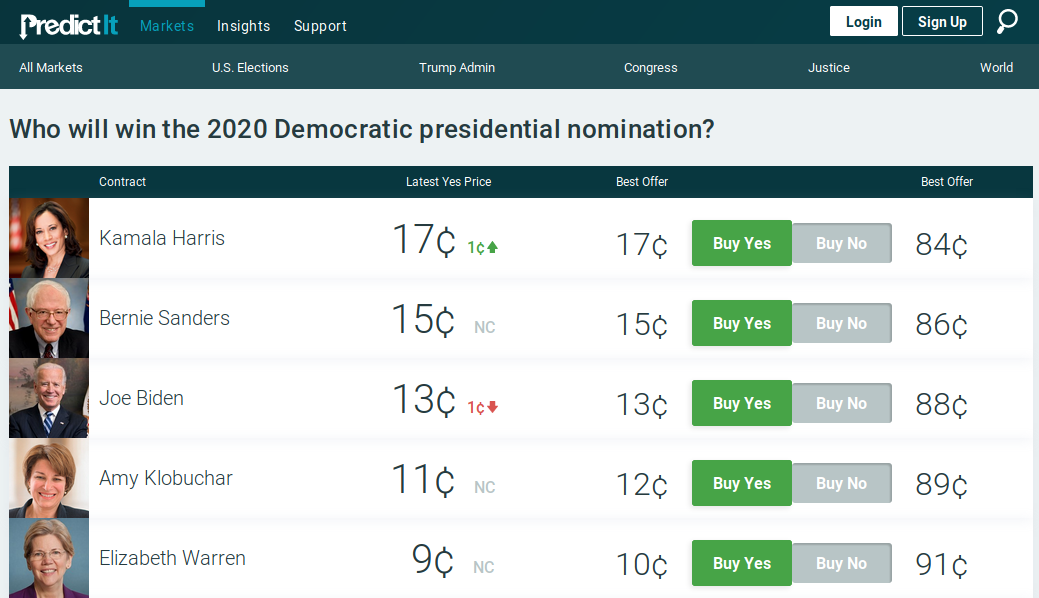
\includegraphics{2020_dem_market.png}
\caption{2020 Dem Primary}
\end{figure}

\end{frame}

\begin{frame}{PredicIt Data}

\begin{figure}
\centering
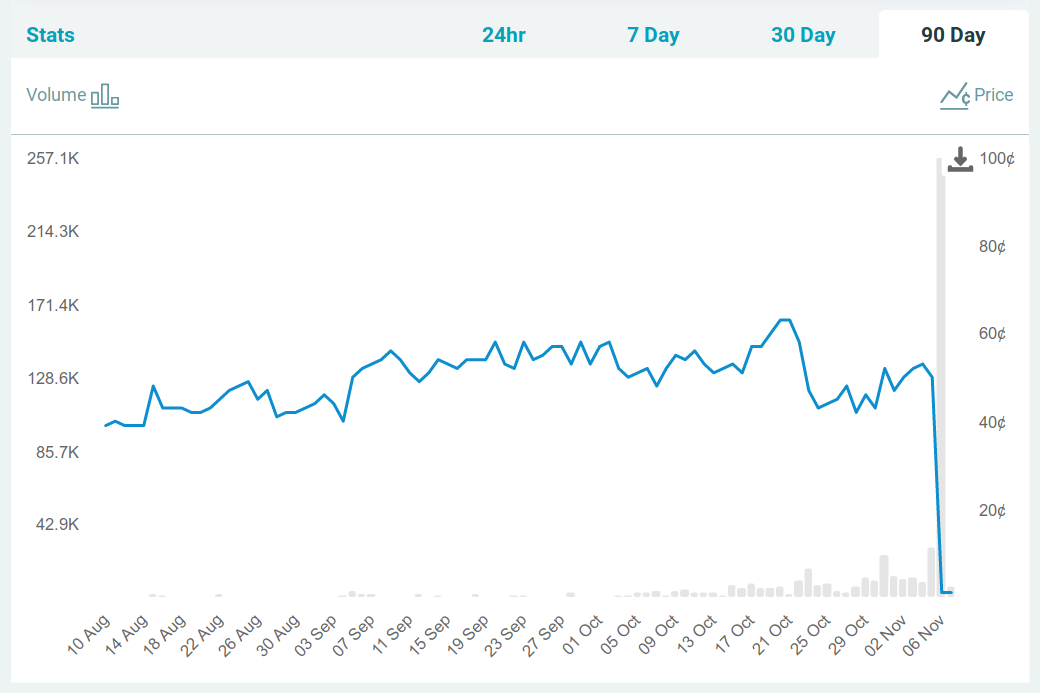
\includegraphics{donnelly_graph.png}
\caption{Donnelly Chart}
\end{figure}

\end{frame}

\begin{frame}{PredictIt Data Collection}

\begin{enumerate}
\def\labelenumi{\arabic{enumi}.}
\tightlist
\item
  Get all active relevant market names from API
\item
  Grab chart data from all above markets
\item
  Merge chart data with API names
\item
  Turn market names into district codes and party affiliation
\end{enumerate}

\end{frame}

\begin{frame}[fragile]{Scraped Market Data}

\begin{verbatim}
## # A tibble: 24,556 x 5
##    date       mid   cid   price volume
##    <date>     <chr> <chr> <dbl>  <dbl>
##  1 2018-08-10 2918  5264   0.95     56
##  2 2018-08-11 2918  5264   0.95     50
##  3 2018-08-12 2918  5264   0.89    100
##  4 2018-08-13 2918  5264   0.9      40
##  5 2018-08-14 2918  5264   0.91     61
##  6 2018-08-15 2918  5264   0.91     85
##  7 2018-08-16 2918  5264   0.91     59
##  8 2018-08-17 2918  5264   0.91      0
##  9 2018-08-18 2918  5264   0.91      0
## 10 2018-08-19 2918  5264   0.95     50
## # ... with 24,546 more rows
\end{verbatim}

\end{frame}

\begin{frame}{Market API Names}

\begin{itemize}
\tightlist
\item
  Which party will win GA-07?
\item
  Which party will win AK at-large?
\item
  Will Brian Fitzpatrick be re-elected?
\item
  Which party will win MS Senate special?
\item
  Will Pelosi be re-elected?
\item
  Will a Dem candidate win the 2018 House of Reps race in WA's 3rd
  district?
\end{itemize}

\end{frame}

\begin{frame}[fragile]{Formatting Names}

\begin{Shaded}
\begin{Highlighting}[]
\KeywordTok{if_else}\NormalTok{(}\KeywordTok{str_detect}\NormalTok{(market_history}\OperatorTok{$}\NormalTok{code, }\StringTok{"re-elected"}\NormalTok{),}
        \KeywordTok{word}\NormalTok{(market_history}\OperatorTok{$}\NormalTok{code, }\DecValTok{3}\NormalTok{),}
\KeywordTok{if_else}\NormalTok{(}\KeywordTok{str_detect}\NormalTok{(market_history}\OperatorTok{$}\NormalTok{code, }\StringTok{"at-large"}\NormalTok{),}
        \KeywordTok{paste}\NormalTok{(}\KeywordTok{word}\NormalTok{(market_history}\OperatorTok{$}\NormalTok{code, }\DecValTok{5}\NormalTok{), }\StringTok{"01"}\NormalTok{, }\DataTypeTok{sep =} \StringTok{"-"}\NormalTok{),}
\KeywordTok{if_else}\NormalTok{(}\KeywordTok{str_detect}\NormalTok{(market_history}\OperatorTok{$}\NormalTok{code, }\StringTok{"special"}\NormalTok{),}
        \KeywordTok{paste}\NormalTok{(}\KeywordTok{word}\NormalTok{(market_history}\OperatorTok{$}\NormalTok{code, }\DecValTok{5}\NormalTok{), }\StringTok{"98"}\NormalTok{, }\DataTypeTok{sep =} \StringTok{"-"}\NormalTok{),}
\KeywordTok{if_else}\NormalTok{(}\KeywordTok{str_detect}\NormalTok{(market_history}\OperatorTok{$}\NormalTok{code, }\StringTok{"Senate"}\NormalTok{),}
        \KeywordTok{paste}\NormalTok{(}\KeywordTok{word}\NormalTok{(market_history}\OperatorTok{$}\NormalTok{code, }\DecValTok{5}\NormalTok{), }\StringTok{"99"}\NormalTok{, }\DataTypeTok{sep =} \StringTok{"-"}\NormalTok{),}
\KeywordTok{if_else}\NormalTok{(}\KeywordTok{str_detect}\NormalTok{(market_history}\OperatorTok{$}\NormalTok{code, }\StringTok{"re-elected"}\NormalTok{),}
        \KeywordTok{word}\NormalTok{(market_history}\OperatorTok{$}\NormalTok{code, }\DecValTok{3}\NormalTok{),}
\KeywordTok{if_else}\NormalTok{(}\KeywordTok{str_detect}\NormalTok{(market_history}\OperatorTok{$}\NormalTok{code, }\StringTok{"Which party"}\NormalTok{),}
        \KeywordTok{word}\NormalTok{(market_history}\OperatorTok{$}\NormalTok{code, }\DecValTok{5}\NormalTok{), }\StringTok{"ERROR"}\NormalTok{))))))}
\end{Highlighting}
\end{Shaded}

\end{frame}

\begin{frame}[fragile]{Market Data Combination}

\begin{verbatim}
## # A tibble: 24,466 x 7
##    date         mid   cid price volume code  party
##    <date>     <dbl> <dbl> <dbl>  <dbl> <chr> <chr>
##  1 2018-08-10  2918  5264  0.95     56 MA-99 D    
##  2 2018-08-11  2918  5264  0.95     50 MA-99 D    
##  3 2018-08-12  2918  5264  0.89    100 MA-99 D    
##  4 2018-08-13  2918  5264  0.9      40 MA-99 D    
##  5 2018-08-14  2918  5264  0.91     61 MA-99 D    
##  6 2018-08-15  2918  5264  0.91     85 MA-99 D    
##  7 2018-08-16  2918  5264  0.91     59 MA-99 D    
##  8 2018-08-17  2918  5264  0.91      0 MA-99 D    
##  9 2018-08-18  2918  5264  0.91      0 MA-99 D    
## 10 2018-08-19  2918  5264  0.95     50 MA-99 D    
## # ... with 24,456 more rows
\end{verbatim}

\end{frame}

\begin{frame}[fragile]{Joining Markets and Models}

\begin{verbatim}
## # A tibble: 24,555 x 6
##    date       code  party  prob price volume
##    <date>     <chr> <chr> <dbl> <dbl>  <dbl>
##  1 2018-08-10 MA-99 D     0.999  0.95     56
##  2 2018-08-10 TX-99 R     0.742  0.7    1303
##  3 2018-08-10 VT-99 D     1      0.95    542
##  4 2018-08-10 WV-99 D     0.859  0.75    533
##  5 2018-08-10 IN-99 D     0.864  0.39     12
##  6 2018-08-10 CA-12 D     1      0.9      51
##  7 2018-08-10 ND-99 D     0.594  0.42     81
##  8 2018-08-10 MO-99 D     0.733  0.47    333
##  9 2018-08-10 WI-99 D     0.977  0.83      0
## 10 2018-08-10 MI-99 D     0.985  0.79    390
## # ... with 24,545 more rows
\end{verbatim}

\end{frame}

\begin{frame}[fragile]{Tidy Data}

\begin{verbatim}
## # A tibble: 45,962 x 5
##    date       code  party tool    prob
##    <date>     <chr> <chr> <chr>  <dbl>
##  1 2018-08-10 AZ-99 R     model  0.272
##  2 2018-08-10 AZ-99 R     market 0.02 
##  3 2018-08-10 CA-12 D     model  1    
##  4 2018-08-10 CA-12 D     market 0.9  
##  5 2018-08-10 CA-22 R     model  0.96 
##  6 2018-08-10 CA-22 R     market 0.65 
##  7 2018-08-10 CA-49 R     model  0.197
##  8 2018-08-10 CA-49 R     market 0.03 
##  9 2018-08-10 CA-99 D     model  0.999
## 10 2018-08-10 CA-99 R     model  0.001
## # ... with 45,952 more rows
\end{verbatim}

\end{frame}

\begin{frame}{Probability Boxplots}

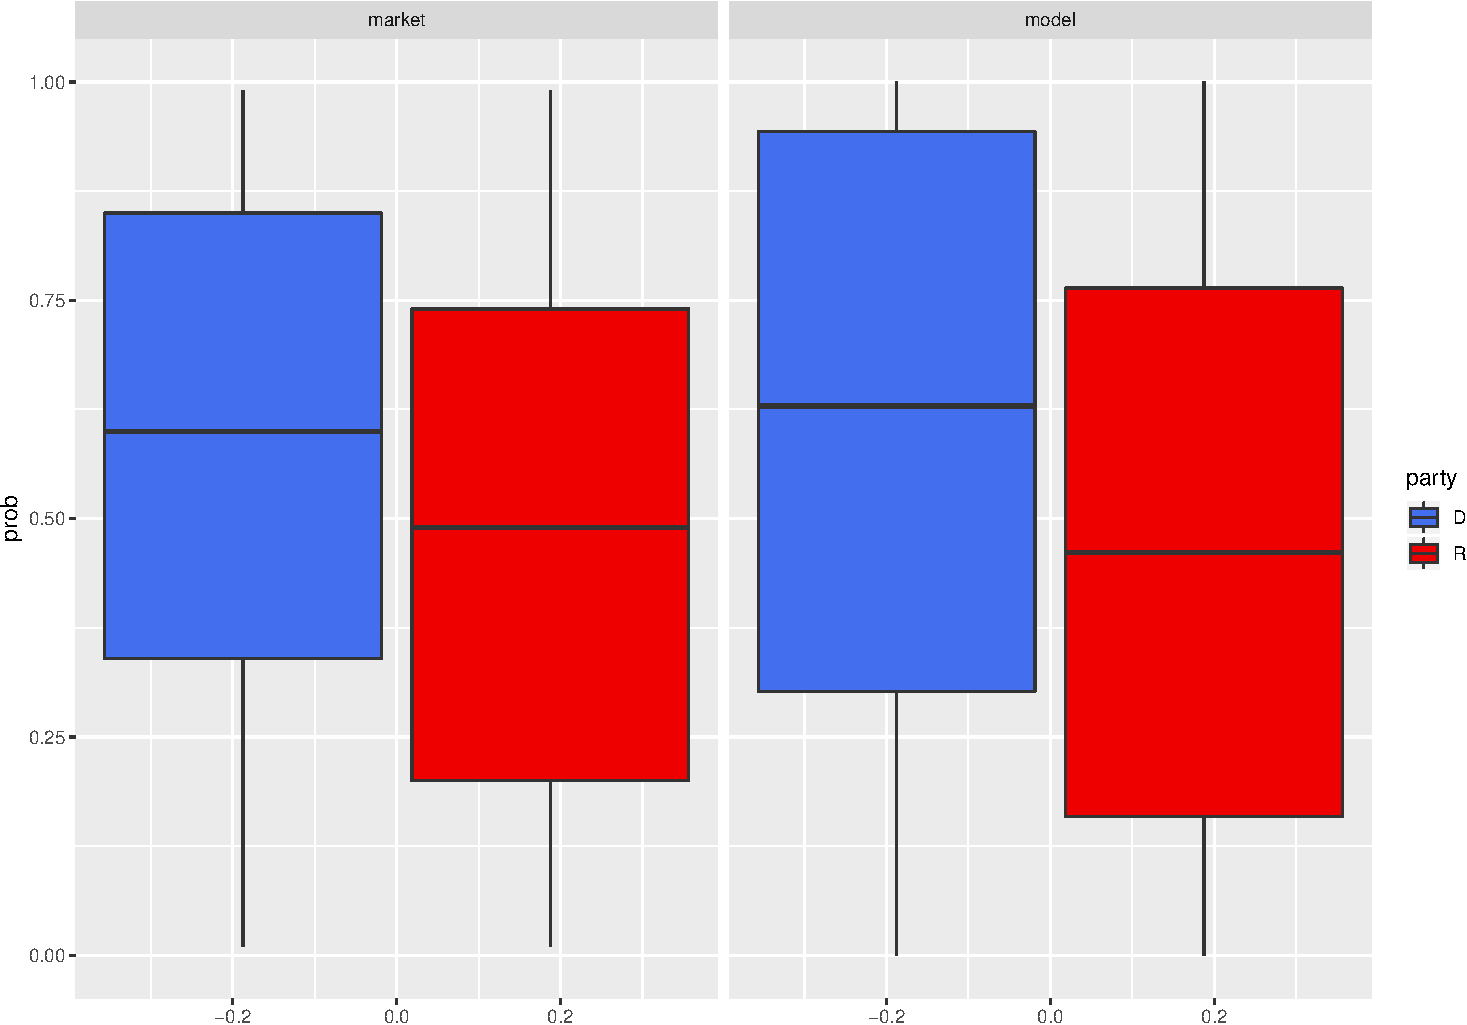
\includegraphics{markets_models_files/figure-beamer/prob box-1.pdf}

\end{frame}

\begin{frame}{Probability Over Time}

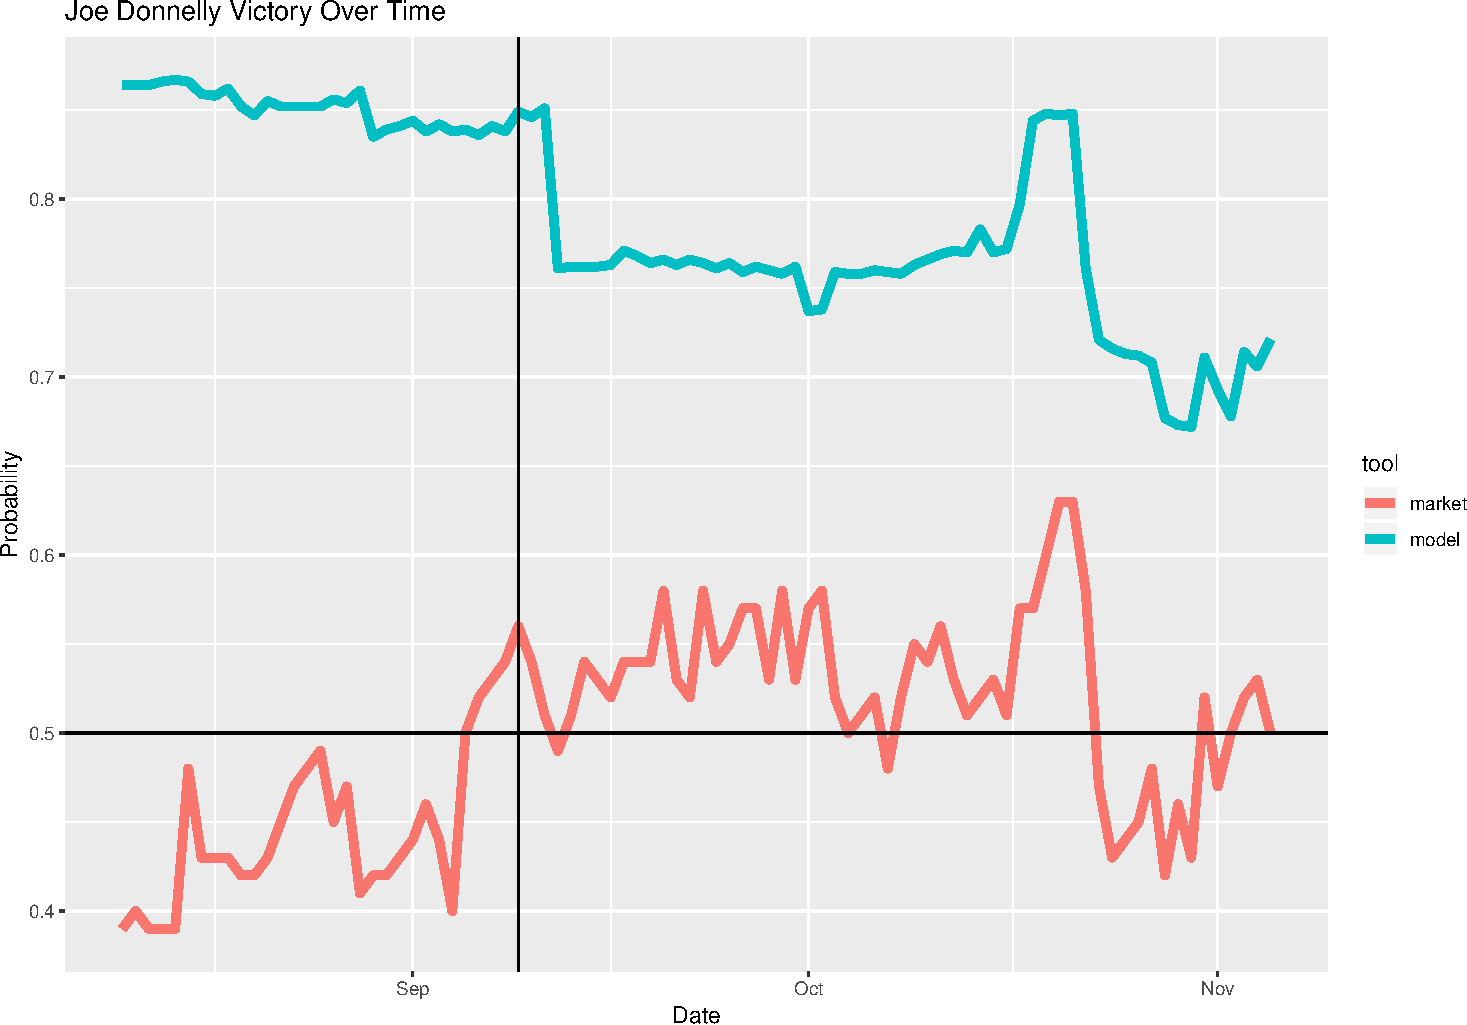
\includegraphics{markets_models_files/figure-beamer/unnamed-chunk-1-1.pdf}

\end{frame}

\begin{frame}{Probability Over Time}

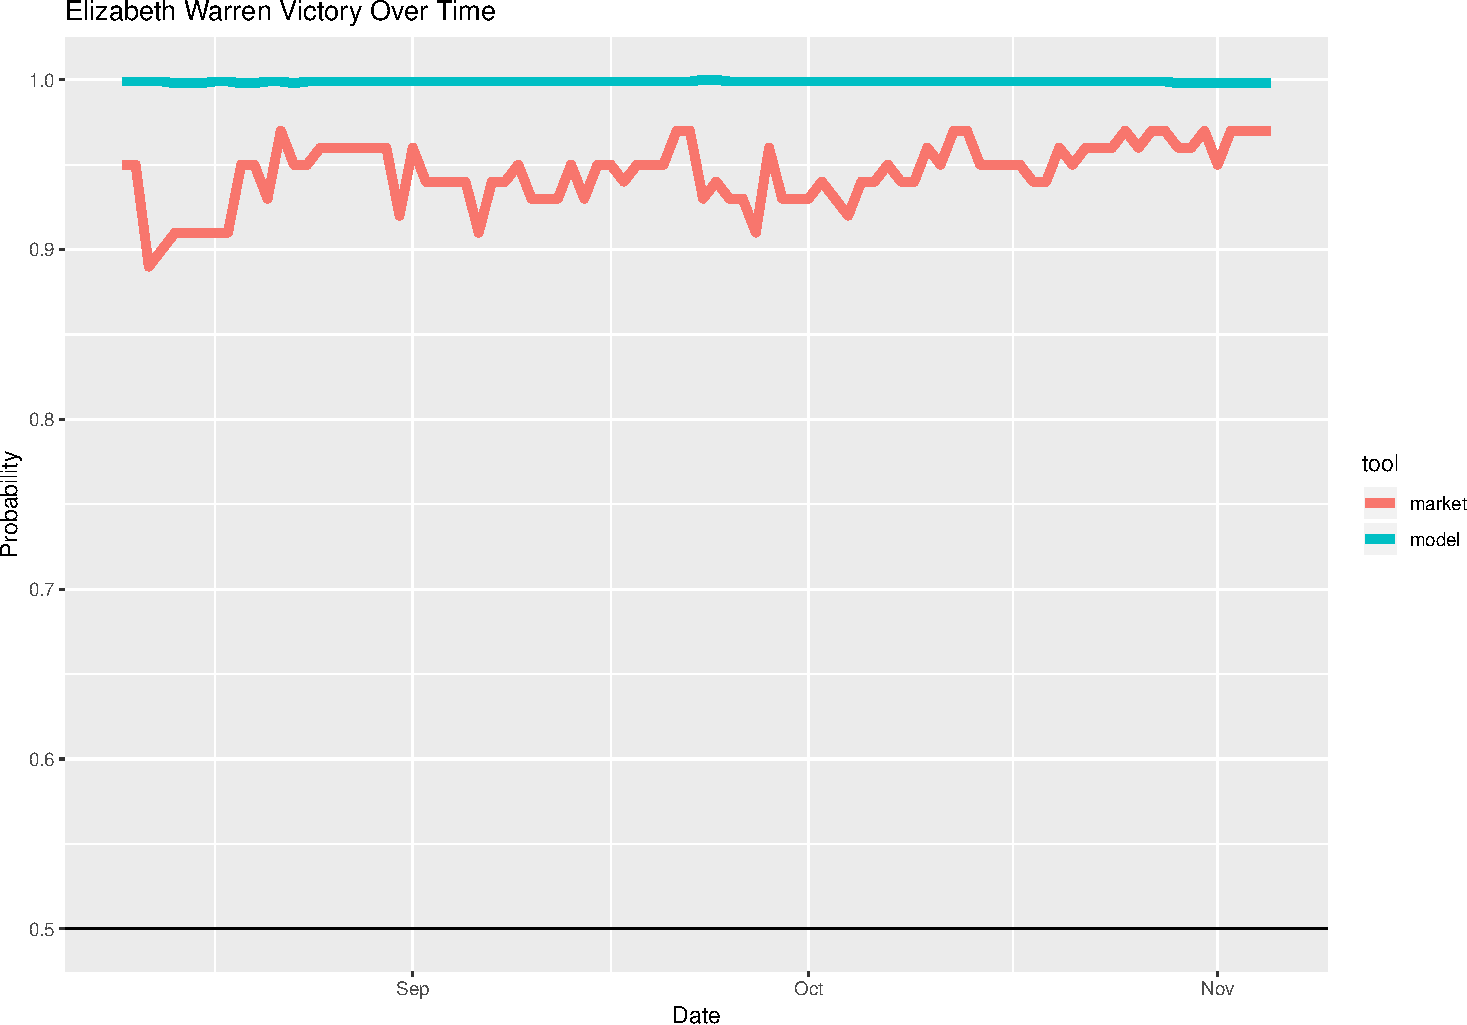
\includegraphics{markets_models_files/figure-beamer/unnamed-chunk-2-1.pdf}

\end{frame}

\begin{frame}{Probability by Tool}

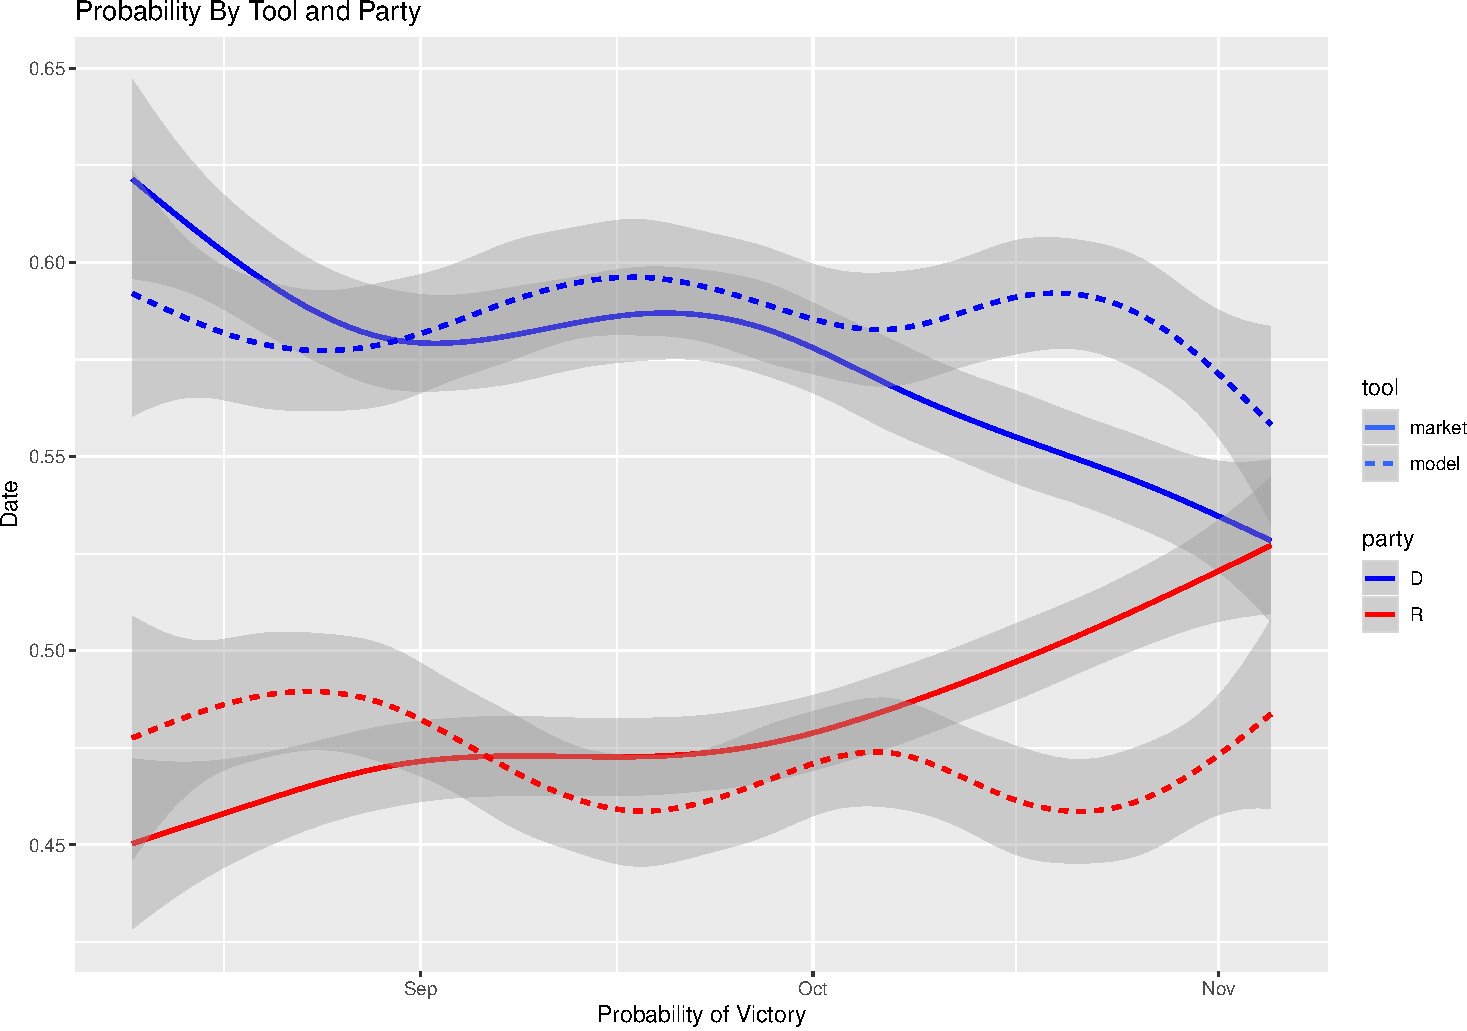
\includegraphics{markets_models_files/figure-beamer/prob tool-1.pdf}

\end{frame}

\begin{frame}{Difference in Tools}

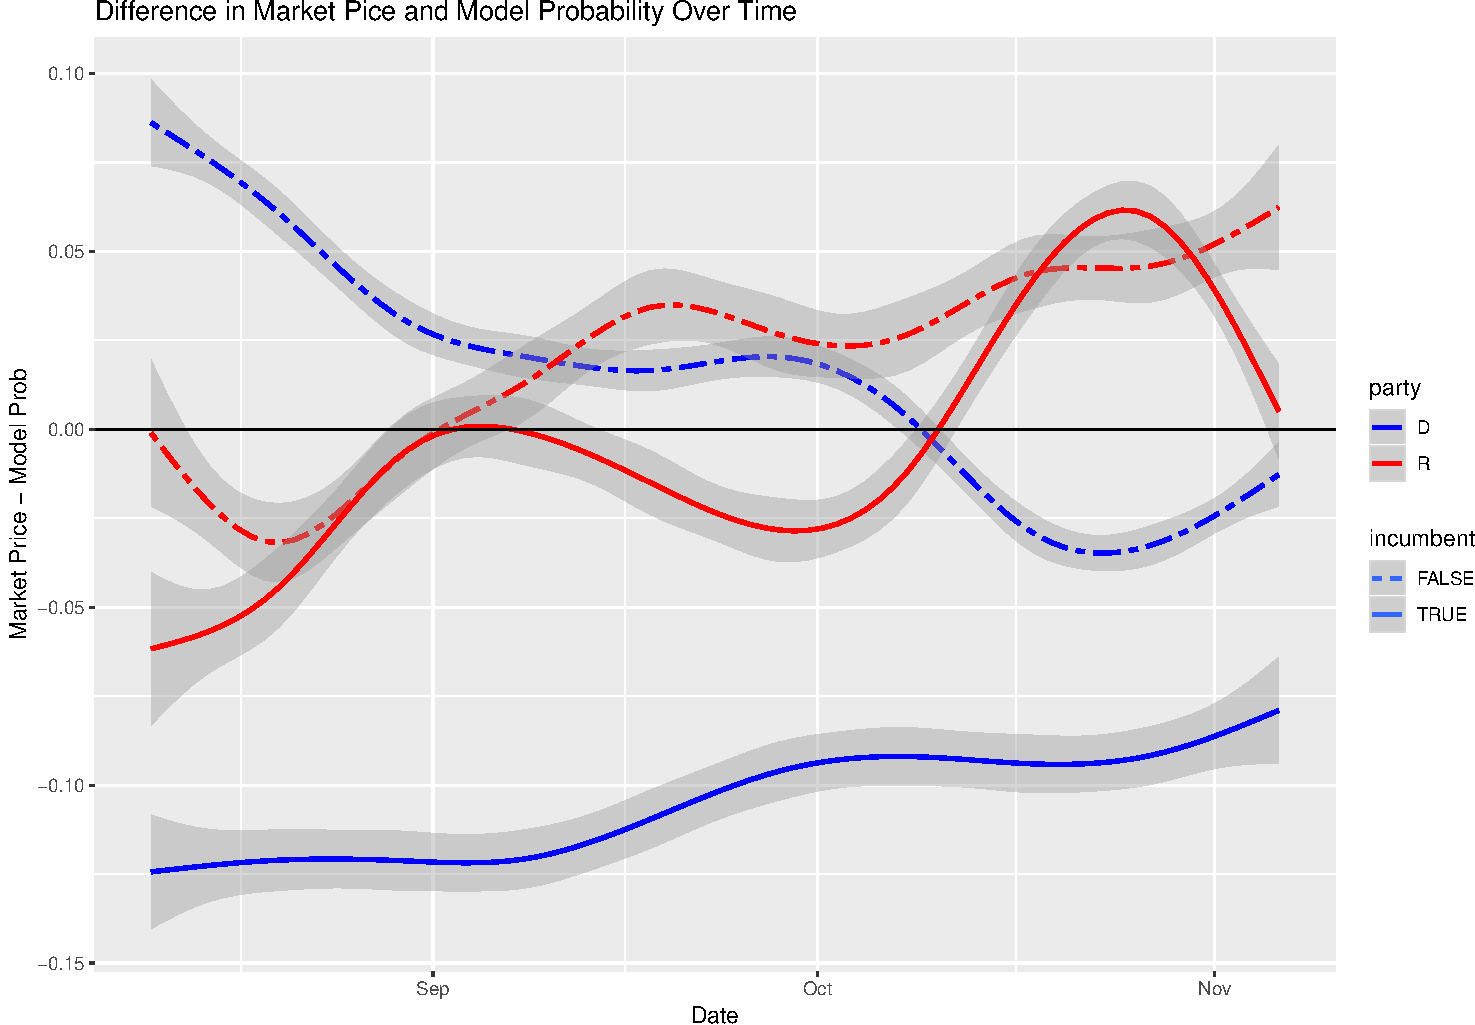
\includegraphics{markets_models_files/figure-beamer/diff-1.pdf}

\end{frame}

\begin{frame}{Difference in Tools}

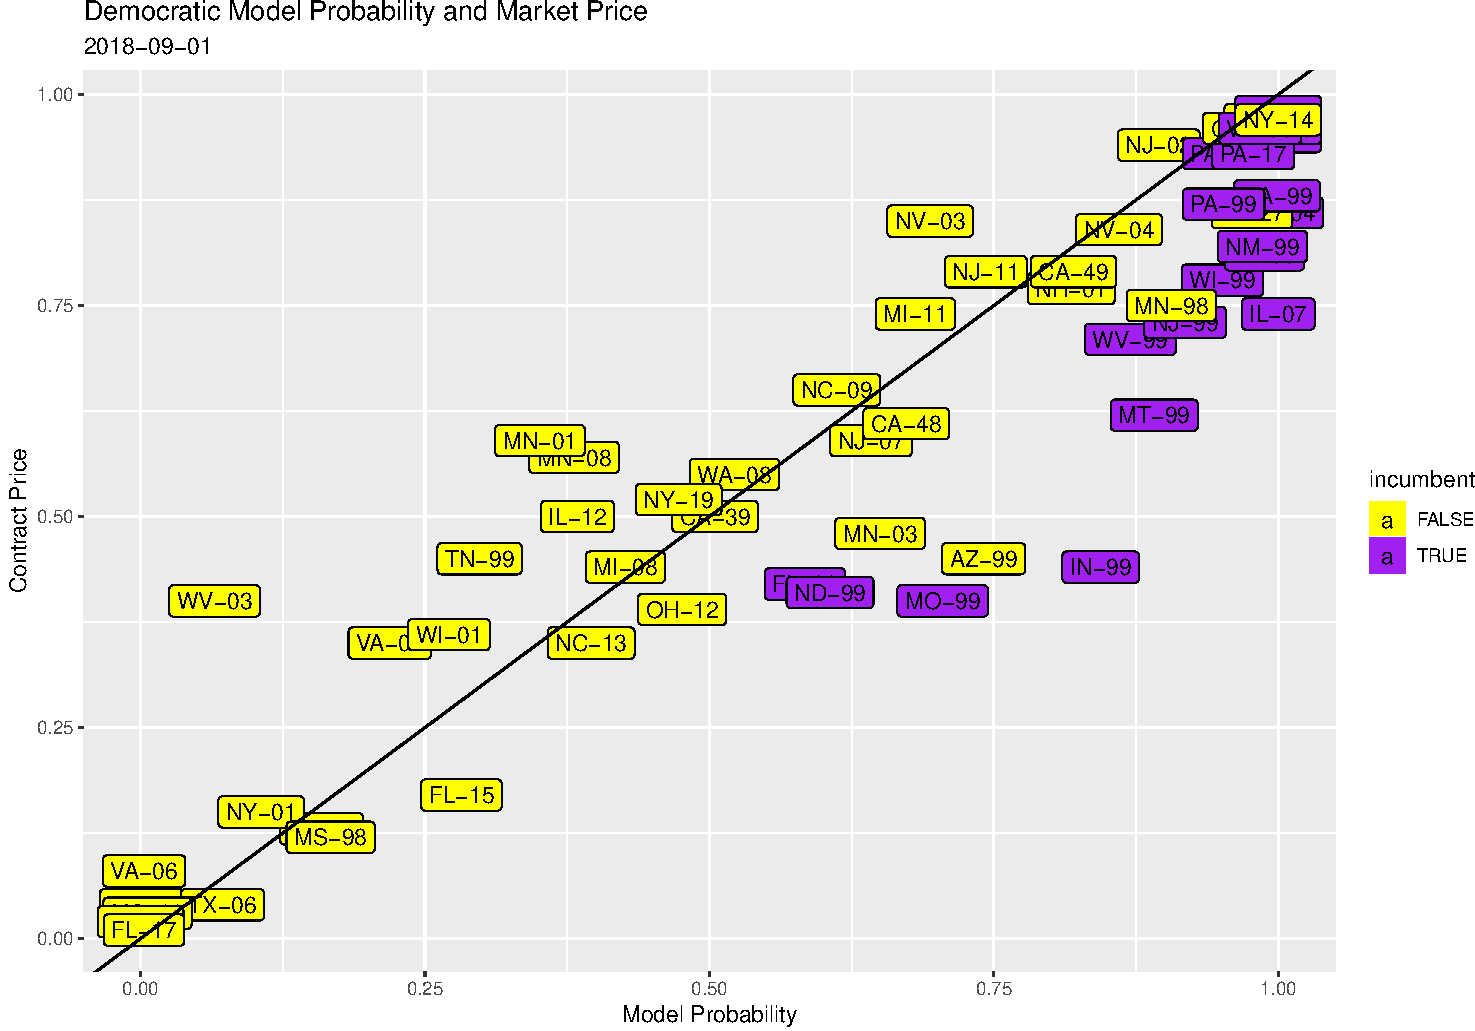
\includegraphics{markets_models_files/figure-beamer/aug10 label-1.pdf}

\end{frame}

\begin{frame}{Difference in Tools}

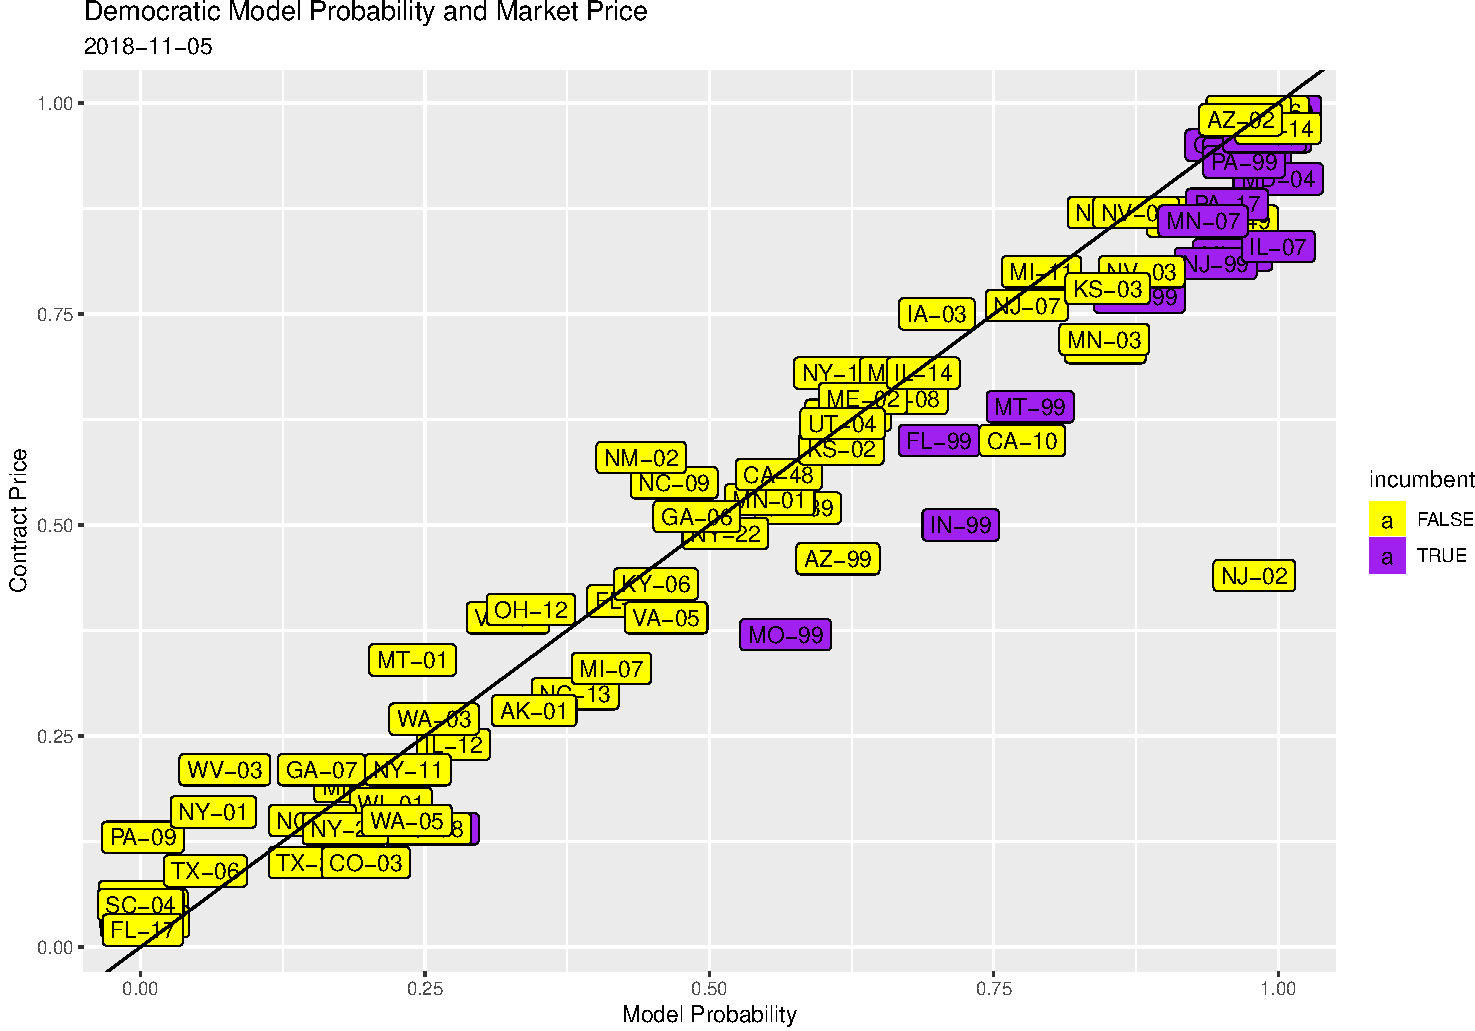
\includegraphics{markets_models_files/figure-beamer/nov05 label-1.pdf}

\end{frame}

\begin{frame}{Weird Markets}

\begin{figure}
\centering
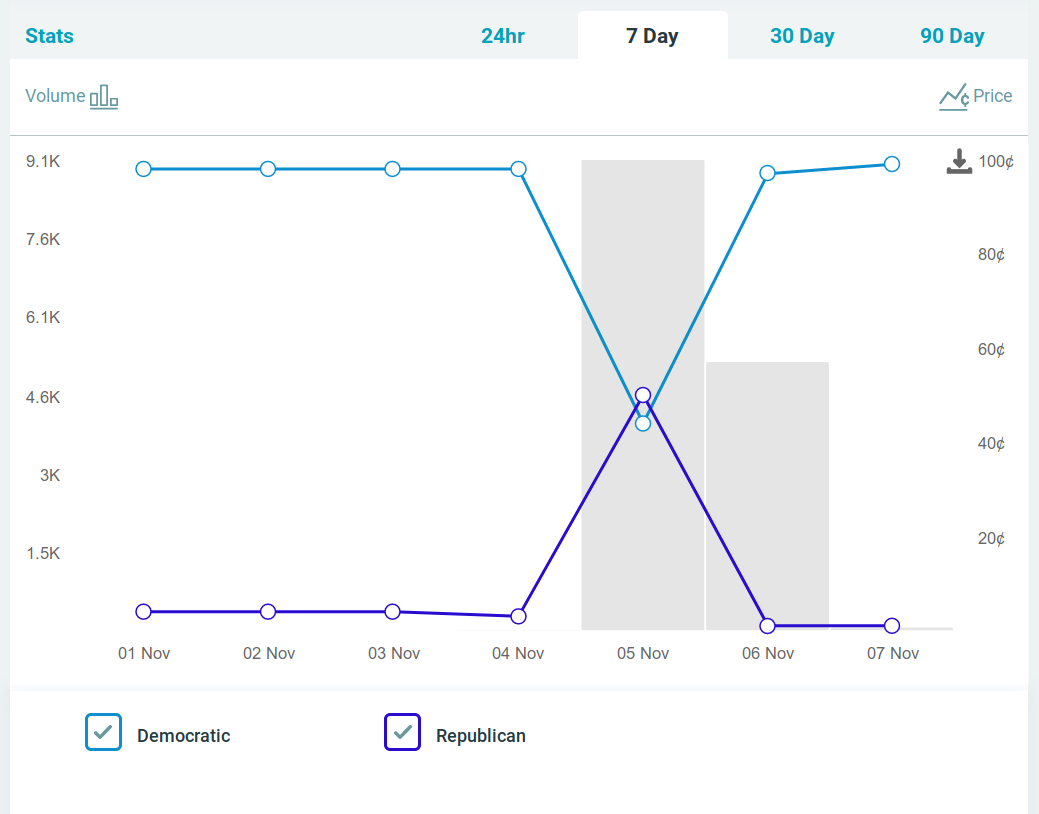
\includegraphics{NJ-02.png}
\caption{NJ-02}
\end{figure}

\end{frame}

\begin{frame}[fragile]{Scraping Results}

\begin{verbatim}
## # A tibble: 470 x 5
##    code    dem   rep class  winner
##    <chr> <dbl> <dbl> <fct>  <chr> 
##  1 AK-01 0.46  0.54  vul R  R     
##  2 AL-01 0.367 0.633 safe R R     
##  3 AL-02 0.385 0.615 safe R R     
##  4 AL-03 0.362 0.638 safe R R     
##  5 AL-04 0.201 0.799 safe R R     
##  6 AL-05 0.389 0.611 safe R R     
##  7 AL-06 0.307 0.693 safe R R     
##  8 AL-07 1     0     safe D D     
##  9 AR-01 0.287 0.69  safe R R     
## 10 AR-02 0.458 0.521 lkly R R     
## # ... with 460 more rows
\end{verbatim}

\end{frame}

\begin{frame}{Cook Race Classifications}

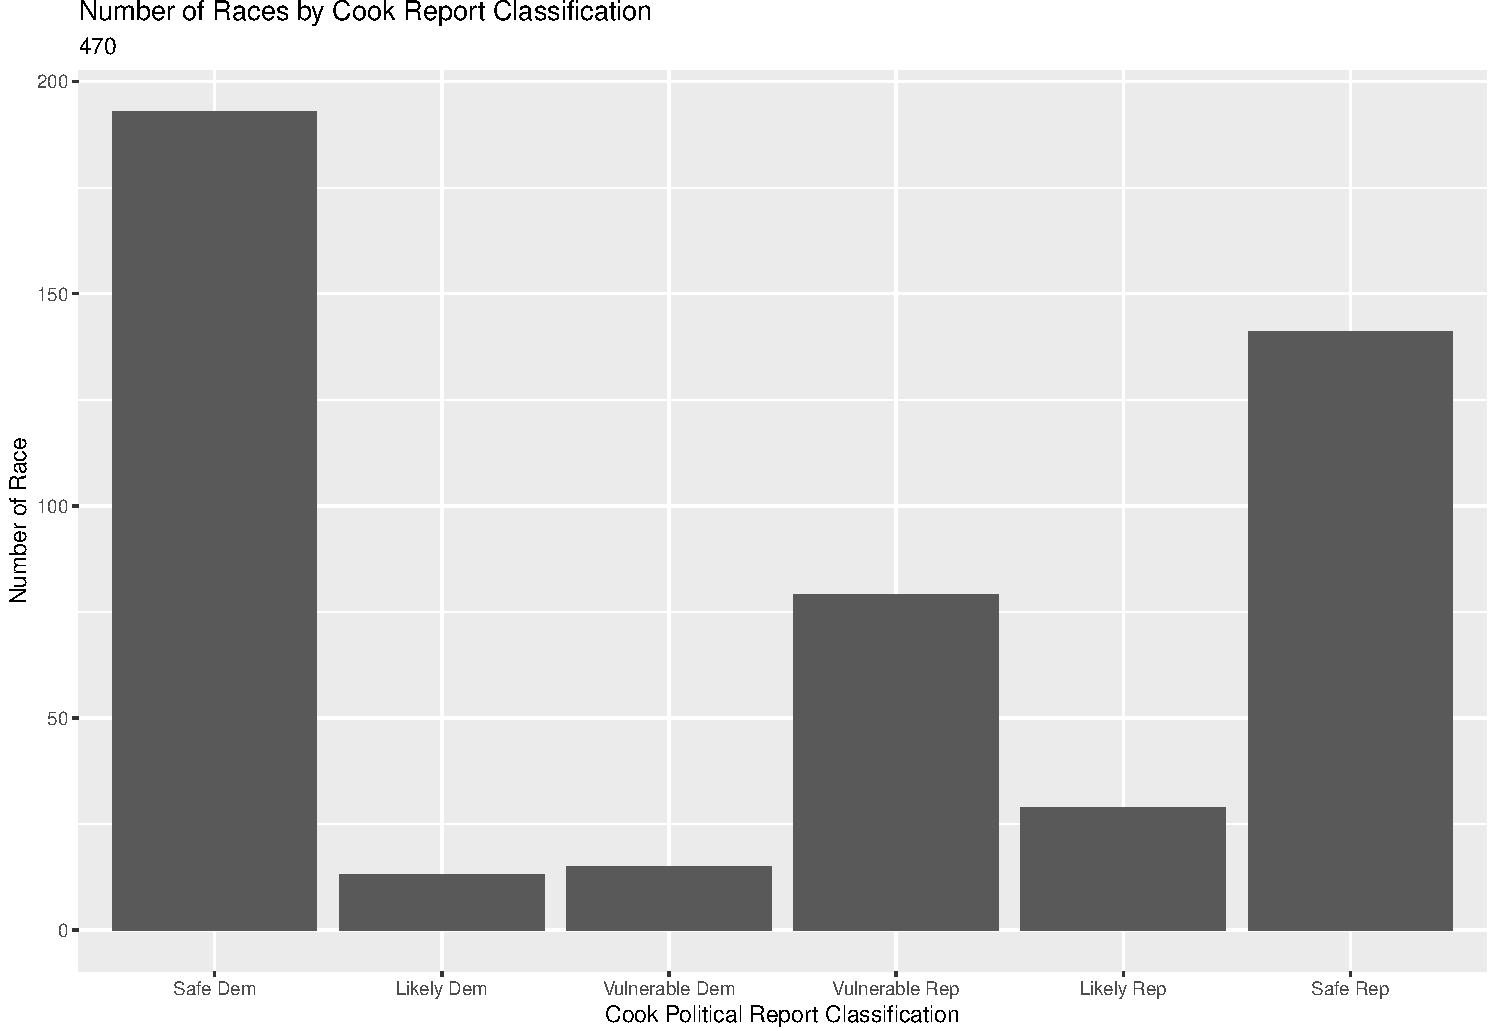
\includegraphics{markets_models_files/figure-beamer/class all-1.pdf}

\end{frame}

\begin{frame}{Cook Race Classifications}

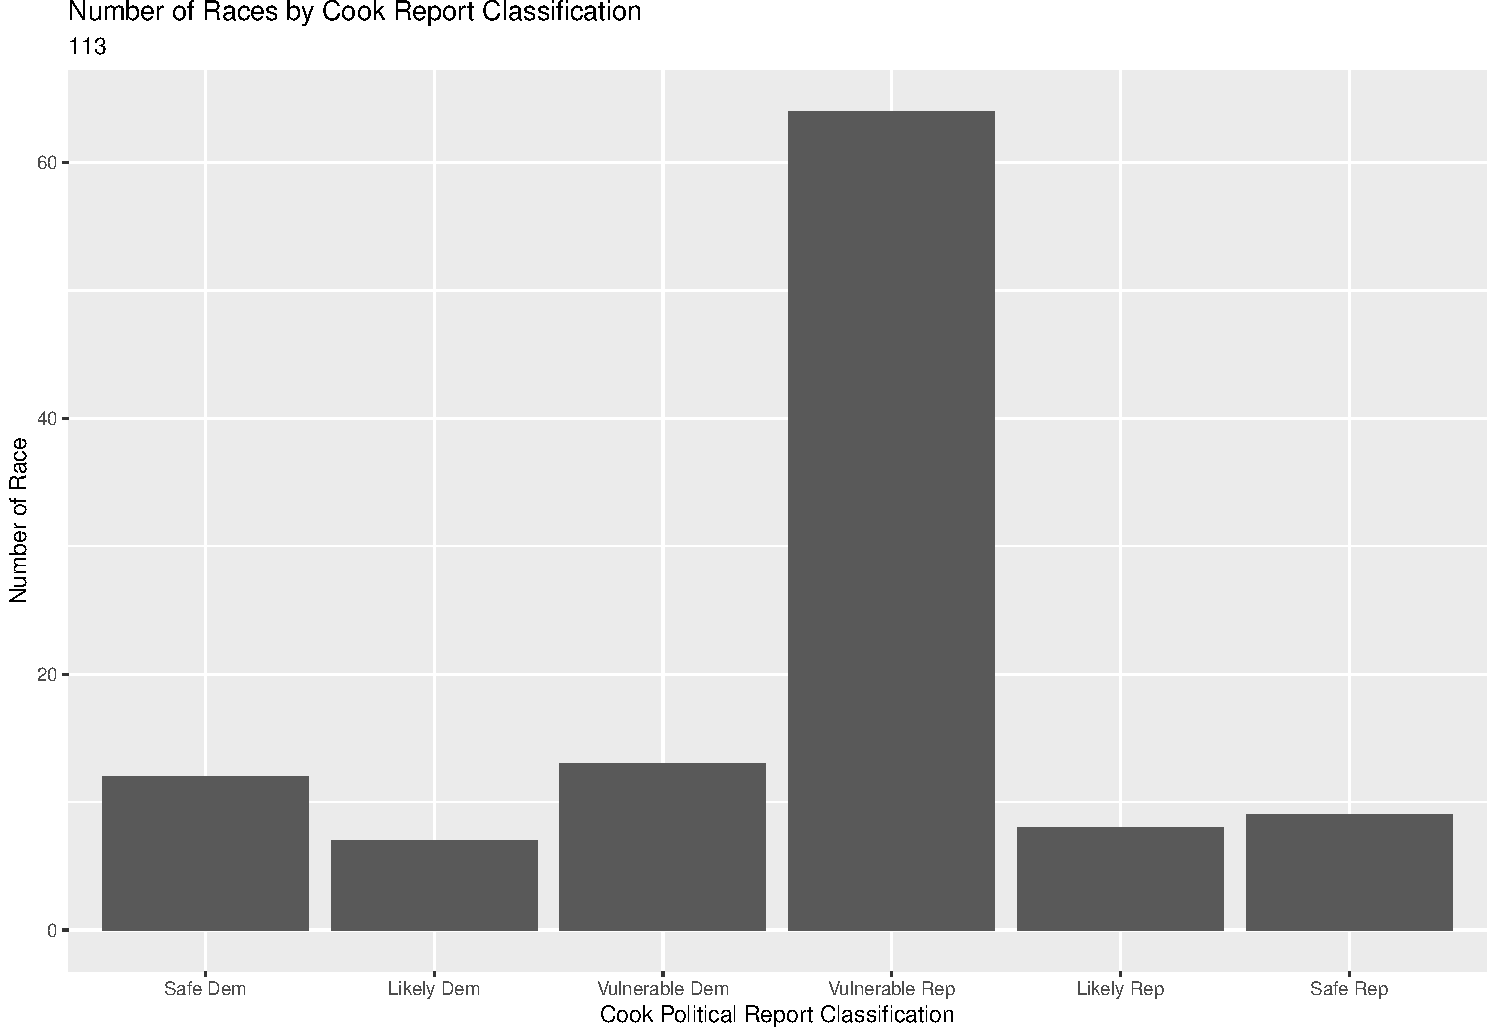
\includegraphics{markets_models_files/figure-beamer/class market-1.pdf}

\end{frame}

\begin{frame}{Post-Election Results}

\begin{enumerate}
\def\labelenumi{\arabic{enumi}.}
\tightlist
\item
  Any given time, \textgreater{} 50\% is a predicted winner
\item
  For each day, ask if guess matches winner
\item
  Average across all races
\item
  Plot over time
\end{enumerate}

\end{frame}

\begin{frame}{Accuracy Over Time}

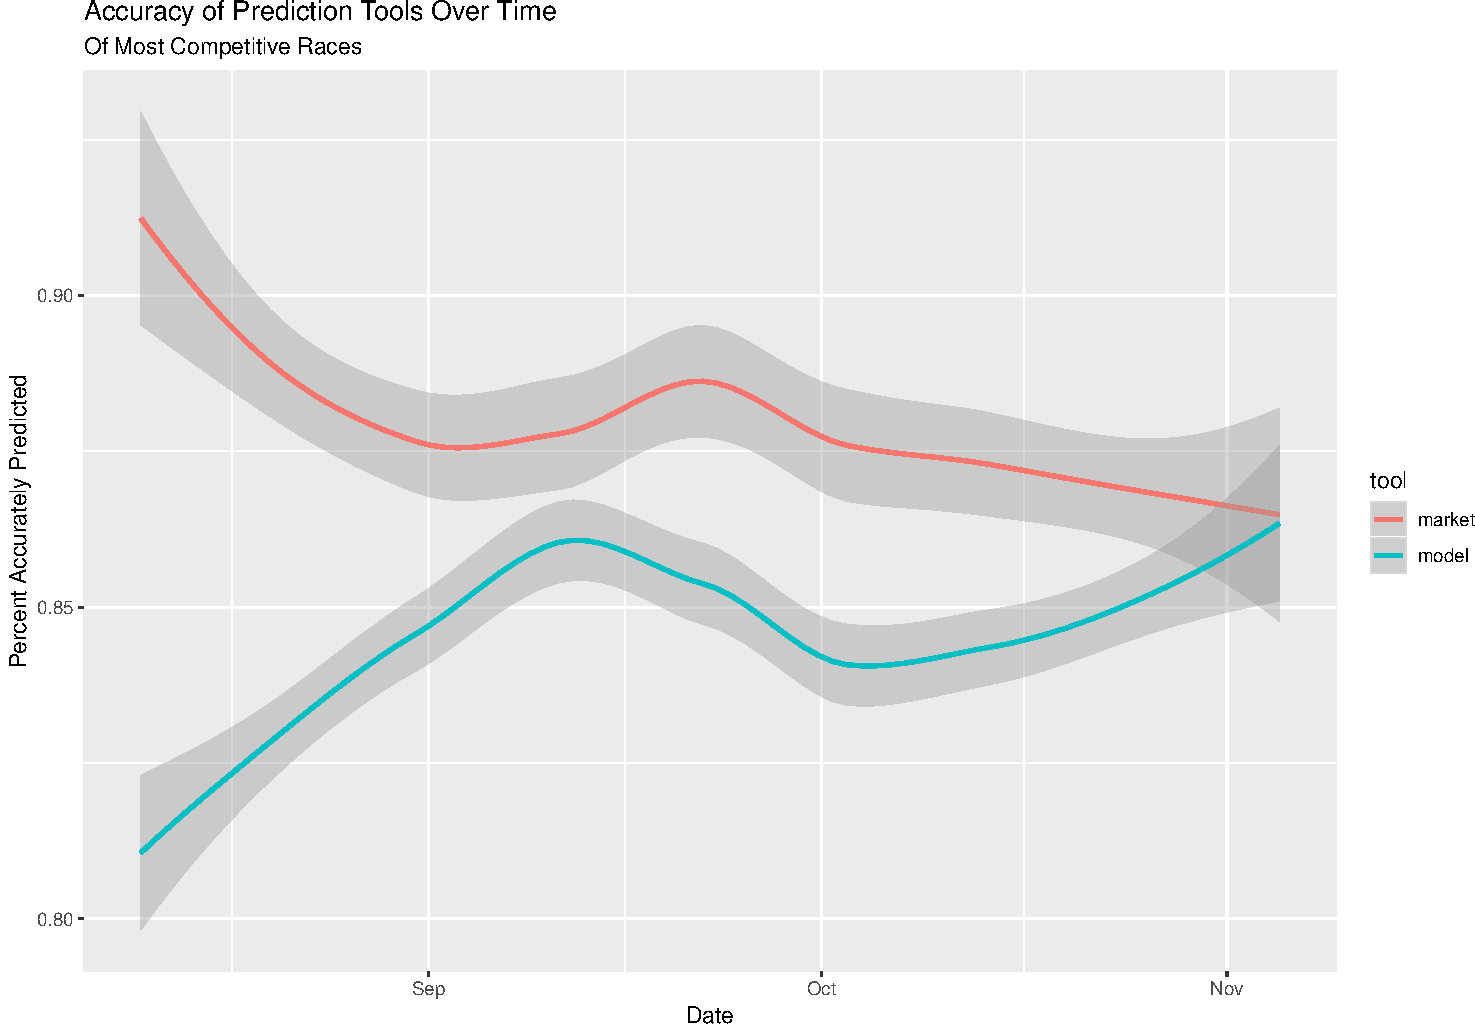
\includegraphics{markets_models_files/figure-beamer/accuracy-1.pdf}

\end{frame}

\begin{frame}[fragile]{Conclusion}

\begin{verbatim}
## # A tibble: 3 x 3
##   day        market model
##   <date>      <dbl> <dbl>
## 1 2018-08-10  0.920 0.851
## 2 2018-09-22  0.908 0.846
## 3 2018-11-05  0.880 0.873
\end{verbatim}

\begin{itemize}
\tightlist
\item
  Methods converge
\item
  With lack of polling, markets have value
\item
  Underestimate Incumbent Democrats
\end{itemize}

\end{frame}

\end{document}
